\begingroup
\titleformat{\chapter}[block]
{\normalfont\Huge\bfseries\centering} 
{Capítulo \thechapter} 
{0.5em}
{: \LARGE}
[\vspace{1em}\titlerule]

\titlespacing*{\chapter}{0pt}{-60pt}{40pt}

\chapter{Introducción}
\label{cap:1_intro}

El objetivo de este primer capítulo es describir el contexto en que está ubicado este Trabajo de Fin de Máster. Explicaremos los problemas que pretendemos resolver usando tecnologías actuales como los modelos de lenguaje a gran escala y los usos que les podemos dar para ayudar a la población. Para ello, marcaremos unos objetivos claros en los que apoyarnos. Por último, presentaremos la estructura que seguirá la memoria.

\section{Motivación}

	Las catástrofes naturales que estamos viviendo estos últimos años, incendios a gran escala o episodios de lluvias torrenciales asociados a Depresiones Aisladas en Niveles Altos (DANA), representan uno de los mayores retos a los que se enfrenta la sociedad actual en el contexto del cambio climático. A finales de pasado año, la Comunidad Valenciana sufrió uno de estos episodios, el cual supuso un punto de inflexión tanto por la intensidad de las precipitaciones como por el impacto social, económico y ambiental que generó \cite{0046_infoDANA}. Calles anegadas, infraestructuras interrumpidas (ver ejemplo en la figura \ref{fig:0000_intro1}), miles de vecinos afectados y un gran volumen de información dispersa en medios de comunicación, redes sociales u organismos oficiales conformaron un panorama en el la correcta gestión y acceso al conocimiento veraz resultaron esenciales \cite{0047_bulosDANA}.
	
	\begin{figure}[H]
		\centering
		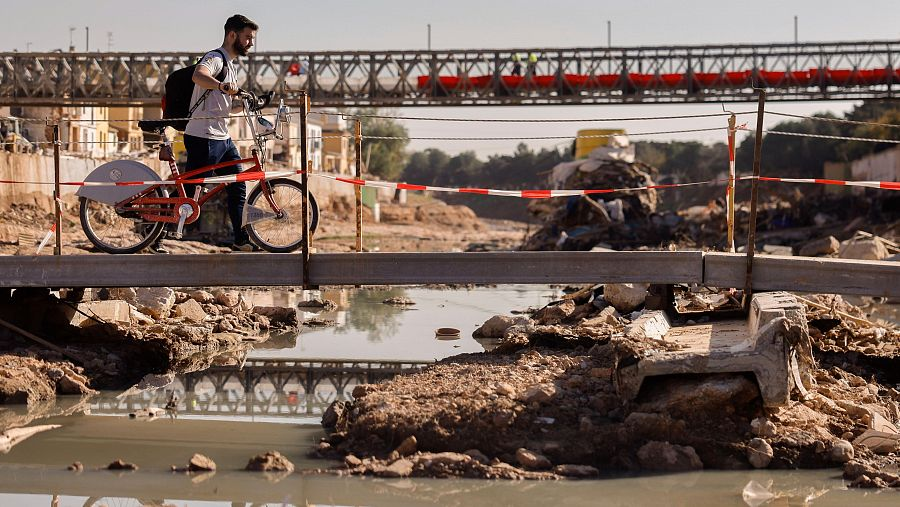
\includegraphics[width=0.8\textwidth]{imagenes/0000_intro1.jpg}
		\caption{Pasarela provisional en la zona del barranco del Poyo en Picanya (Valencia), el 27 de noviembre \cite{0046_infoDANA}}		
		\label{fig:0000_intro1}
	\end{figure} 
	
	\noindent En este contexto, surge la motivación de este Trabajo de Fin de Máster: \textbf{desarrollar un sistema RAG} (Retrieval-Augmented-Generation) (\cite{0003_RAGhowitwork,0003_RAGhowitwork2})  que permita organizar, recuperar y generar información de valor sobre la DANA de Valencia. La elección de este enfoque no es casual, pues las técnicas usadas en un RAG combinan la capacidad de búsqueda eficiente en grandes repositorios de documentos con la generación en lenguaje natural contextualizado y coherente.
	
	\noindent La relevancia social de este trabajo se refuerza por el hecho de que la información utilizada procede de fuentes oficiales, en particular del Boletín Oficial de Estado (BOE) \cite{0048_BOE}. Aunque el BOE constituye la referencia legal sobre ayudas, disposiciones administrativas y medidas de emergencia, su consulta resulta compleja para la mayoría de ciudadanos, más aún en momentos de vulnerabilidad. Una persona afectada por la DANA que necesite conocer qué ayudas solicitar, qué requisitos cumplir o qué plazos respetar se enfrenta a textos jurídicos densos y de difícil navegación. Un sistema RAG aplicado sobre estos documentos permite transformar ese lenguaje administrativo en respuestas claras, comprensibles y accesibles.
	
	\noindent Para hacer efectiva esta idea, el trabajo incluye el \textbf{desarrollo de una interfaz de usuario interactiva}, que permite a cualquier persona formular preguntas en lenguaje natural y recibir respuestas de forma precisa y siempre fundamentadas en la documentación oficial. Esta interfaz no solo es un complemento, sino un componente clave del proyecto, ya que convierte un sistema técnico (como lo es el RAG) en una herramienta práctica con la que cualquier ciudadano, periodista o institución puede interactuar de manera directa. En definitiva, la interfaz actúa como puente entre la complejidad de la inteligencia artificial y la necesidad de simplicidad en la experiencia del usuario final.
	
	\noindent Más allá del desarrollo de una aplicación RAG completa, este TFM también persigue un objetivo de carácter académico y técnico: \textbf{evaluar el sistema RAG} de manera rigurosa mediante métricas específicas. El ámbito de los sistemas RAG es muy dinámico y ofrece múltiples alternativas en cuanto a modelos y algoritmos de recuperación, embeddings y grandes modelos de lenguaje (LLMs). Analizar y comparar diferentes configuraciones resulta fundamental para determinar cuál ofrece el mejor equilibrio entre precisión, coherencia y utilidad práctica. Este segundo objetivo garantiza no solo la validez técnica del trabajo, sino también su capacidad para generar conocimiento transferible a aplicaciones futuras.
	
	\noindent El desarrollo de este proyecto se apoya en la evolución reciente de los modelos de lenguaje (\cite{0005_journeyLLM,0049_tree_evo}), que han alcanzado un nivel de madurez que los convierte en herramientas aptas para aplicaciones de gran impacto social. Muestra de ello es la figura \ref{fig:0000_tree_llm}, donde vemos la gran cantidad de modelos que han ido surgiendo hasta 2023. Los modelos más modernos no solo son capaces de procesar y contextualizar información de manera avanzada, sino que también pueden interactuar con el usuario de manera fluida y natural. Por lo tanto, la integración de estas capacidades en un sistema RAG con interfaz hace posible el diseño de asistentes inteligentes que realmente ayudan en situaciones criticas, consiguiendo a la vez que el ciudadano este informado con fuentes fiables.
	
	\begin{figure}[H]
		\centering
		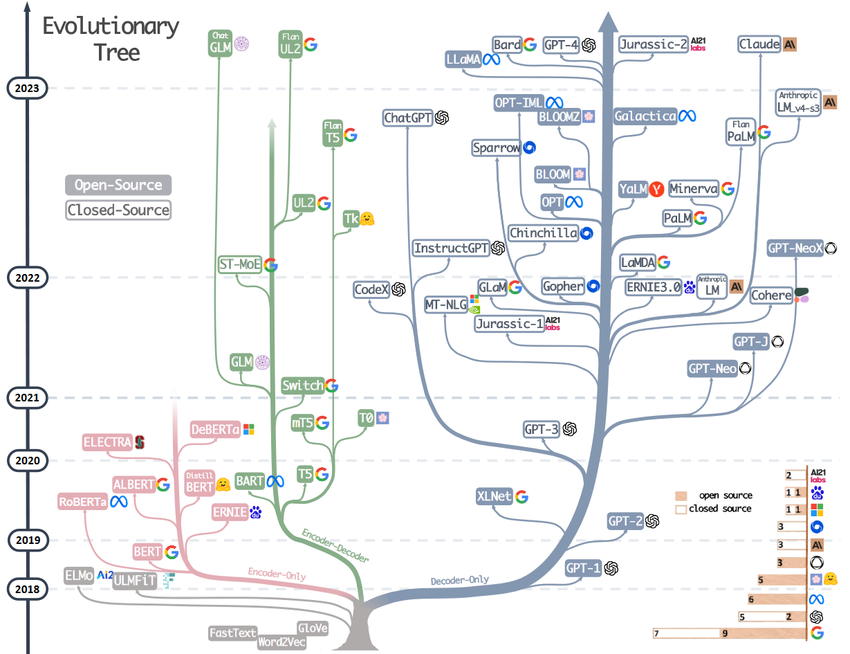
\includegraphics[width=0.8\textwidth]{imagenes/0000_tree_llm.png}
		\caption{Árbol de la evolución de los LLMs modernos \cite{0049_tree_evo}}		
		\label{fig:0000_tree_llm}
	\end{figure} 
	
	\noindent En conjunto, la motivación de este Trabajo de Fin de Máster combina tres vertientes complementarias:
	
	\begin{itemize}
		\item \textbf{Social}, orientada a facilitar el acceso a información oficial a ciudadanos en momentos de crisis ambiental o climática.
		\item \textbf{Práctica}, a través de una interfaz accesible que permite a cualquier usuario interactuar con el sistema RAG sin necesidad de conocimientos previos.
		\item \textbf{Técnica}, centrada en la evaluación comparativa de las diferentes configuraciones que admite un sistema RAG, buscando la máxima eficiencia.
	\end{itemize}
	
	\noindent De este modo, aunque el caso de estudio se centra en la DANA de Valencia de 2024, la metodología y la aplicación desarrollada pueden extrapolarse a otros contextos de crisis. La motivación última es contribuir, desde la investigación universitaria, a un futuro más informado y preparado, en el que la inteligencia artificial actúe como herramienta efectiva para mejorar la vida de la ciudadanía.
	
\section{Objetivos}

	En esta sección comentaremos los dos objetivos definidos para este proyecto: la construcción de un RAG y su evaluación. Describiremos cada uno, desde su justificación hasta su futura implementación.
	
	\noindent El primer objetivo de este trabajo es el desarrollo de un sistema RAG completo, es decir, un sistema que se apoye en información recuperada de una base de conocimiento para generar respuestas más ricas con la ayuda de un modelo de lenguaje. El cometido de nuestro sistema RAG, es el de ayudar a la población a obtener información de cualquier índole (medidas aprobadas, subvenciones, plazos, etc) que esté relacionada con el fenómeno meteorológico DANA, sucedido a finales de 2024.	
	
	\noindent Para este fin, hemos usado documentos del Boletín Oficial de Estado (BOE) relacionados con la DANA para generar nuestra fuente de conocimiento. A partir de aquí, se desarrollará una aplicación con interfaz capaz de recuperar información relevante a la consulta de usuario y de generar una respuesta completa usando esa información. El objetivo es conseguir que nuestro sistema responda con precisión a la duda planteada por la persona en cuestión.
	
	\noindent El segundo objetivo del trabajo, es evaluar el rendimiento de nuestro sistema RAG. Dada la gran cantidad de parámetros ajustables tanto en el modelo de recuperación de información como de elección de modelos de lenguaje para la generación de respuesta, es interesante observar como de distintas son las respuestas ante estos cambios.
	
	\noindent En consecuencia, para la evaluación debemos crear un conjunto de preguntas y respuestas sobre los que aplicar después distintas métricas. Dichas métricas, no son más que \textit{promtps} adaptados que evalúan la precisión, uso de contexto o relevancia de este, en la respuesta generada. Los resultados obtenidos, probando distintas configuraciones en el modelo de recuperación y diferentes modelos de lenguaje, nos indicaran las combinaciones recomendables, o las a evitar.

\section{Estructura de la memoria}

	La estructura de la memoria consta de cinco capítulos finalizando con la bibliografía. El contenido de cada capítulo se describe en la siguiente lista:
	
	\begin{itemize}
		\item \textbf{Capítulo 1. Introducción:} Presenta el proyecto de forma general, explicando la motivación que ha llevado a su realización, los objetivos principales que se persiguen y la organización de la memoria para facilitar su lectura.		
		\item \textbf{Capítulo 2. Estado del Arte:} Revisión de los conceptos teóricos relevantes y descripción de las herramientas, librerías y plataformas empleadas en el desarrollo. Se incluyen además alternativas consideradas, justificando la elección final.		
		\item \textbf{Capítulo 3. Desarrollo del Proyecto:} Exposición del proceso seguido para la construcción de la aplicación RAG, detallando la planificación inicial, la metodología aplicada y las fases de implementación.		
		\item \textbf{Capítulo 4. Evaluación del Proyecto:} Análisis del funcionamiento de la aplicación a partir de métricas y un conjunto de preguntas diseñadas para tal fin. Los resultados se presentan en tablas y gráficas que facilitan su interpretación.		
		\item \textbf{Capítulo 5. Conclusiones y Líneas Futuras:} Recoge las conclusiones generales derivadas del trabajo, así como posibles mejoras y ampliaciones que podrían explorarse en desarrollos posteriores.		
		\item \textbf{Bibliografía:} Relación de las fuentes y referencias consultadas a lo largo de la elaboración del proyecto.
	\end{itemize}
	

\endgroup